

%% ==============
\chapter{Szenario der Heimautomatisierung}
\label{ch:Motivation:sec:Szenario}
%% ===========================
 
Das hier genannte Szenario wird an das Home Automation System Szenario
aus \cite{Pohl2005} angelehnt. Der Komfort der Nutzer sollte sich
durch die Heimautomatisierung steigern. Daraus folgt, dass auch der
Installationsaufwand gering gehalten werden sollte. Der Nutzer ist in
diesem Szenario der einzige Stakeholder, es wird davon ausgegangen,
dass er die Initiative f�r die Anschaffung des Systems hat. Die
Heimautomatisierung deckt viele Bereiche des Lebens und des Hauses. Um
das Anwendungsfeld zu begrenzen wird ein Ausschnitt aus einer
Ubiquit�ren Anwendung f�r das eigene Heim betrachtet. Es werden nur
die im Folgenden aufgef�hrten Komponenten in Betracht genommen:
\begin{itemize}
  \item Regelger�te f�r Heizk�rper
  \item Sensoren und Aktuatoren f�r Fenster
  \item Ein LED-Strang
  \item Steckdosenaufs�tze
  \item Server
  \item Installationsger�t (Smartphone, Tablet, Rechner)
\end{itemize}
% [Graphik cu elemenetele care o sa le contina - fa-le dragutze, diagrame din
% carte ai putea refolosi]
Des Weiteren k�nnten Infrarotsensoren eingesetzt werden um Benutzer im
Raum aufzusp�ren, die dem Konfigurationssystem erlauben
Raumempfehlungen zu geben. Es werden keine anderen Ausgabeger�te, wie
z.B. Bildschirme, benutzt, au�er der Web-Oberfl�che die von
verschiedenen Ger�ten ansteuerbar ist. Eine weitere Randbedingung ist,
dass keine Entertainment Funktionen, wie zum Beispiel Multi-Media
Streaming, betrachtet werden. Es werden keine Sicherheitsaspekte wie
das Nutzer-Management in Betracht gezogen. Das hei�t alle Benutzer in
diesem Szenario haben vollen Zugriff auf das System.
Es werden keine Sicherheitskritischen Anwendungen wie
Gesundheitsmonitoring oder Heimsicherung. Das Sytem hat als Haupt
Anwendungspunkt das Monitoring und Kontrolliern von Temperaturen und Stromfluss. Die Installation laut
dem Generierten Handbuch ist die Forschungsfrage.

Das Heim-Gateway ist der Zentrale Server des Intelligenten Hauses
\cite{Pohl2005}. Anstatt einen Cloud-basierten Ansatz zu fahren wird
der Gateway-Server als zentraler Server f�r die Kommunikation,
Koordination und Datenhaltung dienen. Auf diesem Server kann das
Modell der Anwendung, so wie sie auf den Benutzer zugeschnitten ist
gespeichert und verwaltet werden. Des weiteren soll das Home Gateway
den Code verteilen, die Dokumentation auf dem neuesten Stand halten?
Auf dem Home-Gateway Server werden folgende Daten �ber alle Komponenten des
Systems (\emph{Sensoren, Aktuatoren, Kontrolleinheiten})
abgespeichert:
\begin{itemize}
  \item Informationen �ber die Art und Typ einer Komponenten
  \item Physische Position
  \item Semantische Assoziation
  \item Konfigurationsparameter
 % \item Regeln(workflows) [bazat pe paperu care inca nu l-ai citit, sau poate
 % gasesti ceva generic: k trebe sa existe reguli de control in absenta AI]
\end{itemize}

Variabilit�t in der Heimautomatisierung bedeutet, dass verschiedene
Varianten des Produkets an die Endkunden kommen und diese auf
unterschiedliche Weise Installiert werden m�ssen.
Die verschieden M�glichkeiten Sensoren und Aktuatoren zu kombinieren,
kann die Assoziation und die verschiedenen Steuerungsalgorithmen
�ndern.

\begin{figure}[htp]
\begin{center}
  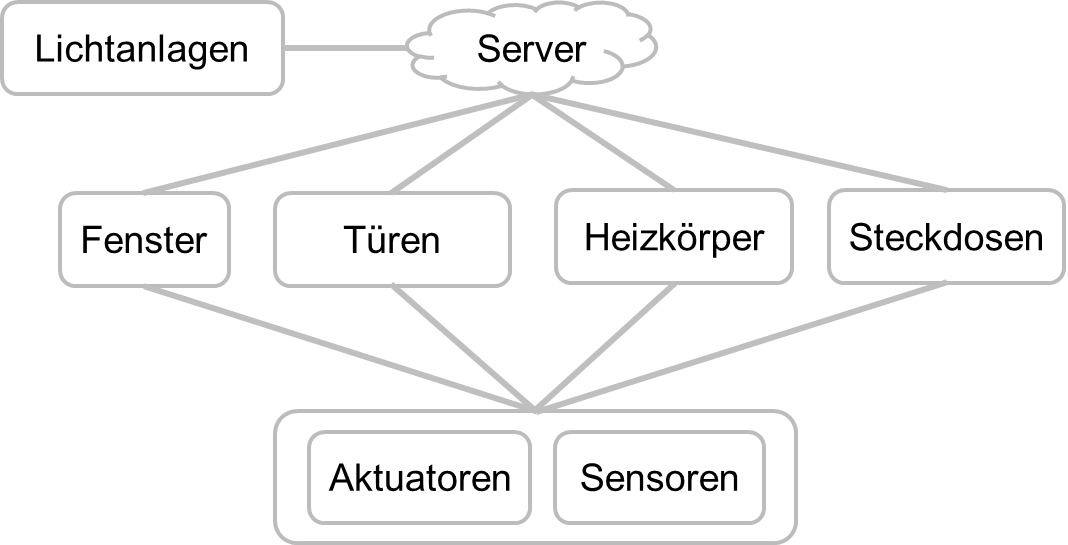
\includegraphics[width=1\textwidth]{img/szenario.png}
  \caption[labelInTOC]{figureCaption}
  \label{figureLabel}
\end{center}
\end{figure}

Die Erstellung der Assoziationen zwischen den Heimautomatiesierungsger�ten und
den von ihnen beobachteten Subjekten wird die Aufgabe des Anwenders
sein.
 
 % Design und Implementierungsentscheidungen werden oft gemacht weil\ldots
 % din cartea cu design of everyday things 
 
 
% Es ist wichtig den Benutzern zu erkl�ren was die Ger�te machen, was
% diese gemacht haben und wie sie kontrolliert werden k�nnen um das
% "debuggen" (z.B. fehlerhafte Assozierungen) durch den Benutzer zu
% erm�glichen \cite{Edwards2001}.
% Dies gilt besonders im Fall in dem neue Ger�te dazukommen, alte
% entfernt werden oder die Ger�te von unterschiedlichen Herstellern
% kommen.

% Das System soll durch Web-Oberfl�chen kontrolliert werden.